\documentclass[10pt]{article}
\usepackage{mathpaper}

\begin{document}
\papertitle{第二十二章~~~二次函数}
\paperinformation{时间:2小时~~~~满分:120分}
\informationline
\begin{questions}{\selectingintroduction}
    \question 下列函数为二次函数的是(~~~~~~~)
    \twp{$y = x^{2} - 2x + 1 - (x - 1)(2x + 1)$}{$y = \frac{x^{4} - 3x^{3} + x^{2} + 1}{x}$}{$y = 18x - 16$}{$y = x^{2} + 2x + 3 - \frac{1}{x}$}
    \question 二次函数$y = x^{2} + ax + 1 - a$的图像必过点(~~~~~~~)
    \onp{$(0,1)$}{$(1,2)$}{$( - 1,0)$}{$(0,0)$}
    \question 若二次函数$y = x^{2} + 4x + 4$的图像与一次函数$y = ax + a$的图像有且仅有一个交点,则(~~~~~~~)
    \onp{$a = 2$}{$a = 4$}{$a = - 1$}{$a = - 2$}
    \question 已知二次函数$y = ax^{2} + bx + c$的顶点为$(4, - 2)$,且过点$(6,2)$,则(~~~~~~~)
    \twp{$a = - 1,b = 8,c = 18$}{$a = 1,b = 8,c = 14$}{$a = 1,b = - 8,c = 14$}{$a = - 1,b = 6,c = - 14$}
    \question %5
    \question %6
    \question %7
    \question %8
    \question 若关于$x$的一元二次方程$ax^2-2ax-2=0$在$-1<x<4$范围内有且仅有一根,则实数$a$的取值范围是(~~~~~~~)
    \onp{$a > \frac{2}{3}$}{$a < \frac{1}{4}$}{$\frac{1}{4} < a < \frac{2}{3}$}{$a > \frac{2}{3}$或$a < \frac{1}{4}$}
    \question 如图,在平行四边形$ABCD$中,$BC=2AB=20$,$B$、$F$、$E$三点共线,且$\angle ABC=60^{\circ}$.连$AF$、$AE$、$CE$,若$AE=EF$,$\angle DAE+\angle CBF=60^{\circ}$,且$AF=6$,则$\Delta BEC$的面积为(~~~~~~~)
    \onp{$16\sqrt{3}$}{$68\sqrt{3}$}{$32\sqrt{3}$}{$34\sqrt{3}$}
    \begin{figure}[htb]
        \centering
        \raggedleft
        \subfigure[(第10题)]{
        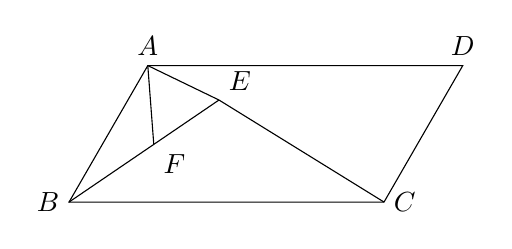
\begin{tikzpicture}[scale=0.4]
            \coordinate[label=above:{$A$}] (A) at (2.5,4.33333);
            \coordinate[label=left:{$B$}] (B) at (0,0);
            \coordinate[label=above:{$D$}] (D) at (12.5,4.33333);
            \coordinate[label=right:{$C$}] (C) at (10,0);
            \coordinate[label=above right:{$E$}] (E) at (4.76,3.24);
            \coordinate[label=below right:{$F$}] (F) at (2.69,1.83);
            \draw (A)--(B)--(C)--(D)--cycle;
            \draw (A)--(F);
            \draw (A)--(E);
            \draw (C)--(E);
            \draw (B)--(E);
        \end{tikzpicture}}
    \end{figure}
\end{questions}
\begin{questions}{\complitingintroduction}
    \question 抛物线$y = 4x^{2} + 6x + 2$与$x$轴的交点是\complitingline\complitingline.
    \question 二次函数$y = x^{2} + 6x + 7$的顶点为\complitingline.
    \question 已知实数$a$、$b$、$c$满足$a \neq 0$,且$a - b + c = 0$、$9a + 3b + c = 0$,则抛物线$y = ax^{2} + bx + c$图像上一点$A( - 1,3)$关于抛物线对称轴对称的点为\complitingline.
    \question 把二次函数$y = ax^{2} + bx + c\ (a > 0)$的图像作关于$x$轴的对称变换,所得图像的解析式为$y = - a(x - 1)^{2} + 4a$,若$(m - 1)a + b + c \leq 0$,则$m$的最大值为\complitingline.
    \question 如图,抛物线$y = ax^{2} + bx + c (a \neq 0)$的对称轴为直线$x = - 1$,则有下列说法:
    \begin{subsubquestions}
        \subsubquestion $abc < 0$;
        \subsubquestion $3a + c > 0$;
        \subsubquestion $\left( \frac{b}{a} \right)^{2} - \frac{4c}{a} > 4$;
        \subsubquestion 当抛物线经过点$\left( \frac{1}{2},2 \right)$时,若方程$ax^{2} + bx + c - 2 = 0$的两根为$x_{1},x_{2}\left( x_{1} < x_{2} \right)$,则$x_{1} + x_{2} = - \frac{3}{2}$;
        \subsubquestion 若在方程$\left| ax^{2} + bx + c \right| = k$中,$k$为常数,且$0 < k < - a + b - c$,则方程所有根的和为$- 4$;
    \end{subsubquestions}
    其中正确的有\complitingline\complitingline.
    \begin{figure}[htb]
        \centering
        \raggedleft
        \subfigure[(第15题)]{
        \begin{tikzpicture}[scale=0.35,>=Stealth]
            \draw[->] (-5.75,0) -- (2.2,0) node[below] {$x$};
            \draw[->] (0,-5.2) -- (0,5.2) node[right] {$y$};
            \draw (-1.6,0.1)--(-1.6,0) node[below] {$-1$};
            \draw (1.6,0.1)--(1.6,0) node[below] {$1$};
            \draw (-4.9333333333,5) parabola bend (-1.6,-5) (1.7333333333,5);
        \end{tikzpicture}}
    \end{figure}
    \question 若关于$x$的方程$ax^2-3x-1=0$的所有实根均满足$-1<x<0$,则$a$的取值范围是\complitingline.
\end{questions}
\begin{questions}{\answeringintroduction}
    \question 已知在平面直角坐标系内有一条抛物线过点$(-2,2)$、$(3,2)$和$(2,-4)$,求这条抛物线的顶点坐标.
    \question %18
    \begin{subquestions}
        \subquestion %18.1
        \subquestion %18.2
    \end{subquestions}
    \question 已知二次函数$y=x^2+ax+2a$的图像与$x$轴有两个交点,且这两个交点间的距离为$3$.
    \begin{subquestions}
        \subquestion 求$a$.
        \subquestion 试讨论当$b \le x \le b+5$时,函数值$y$的最小值.
    \end{subquestions}
    \question
    \begin{subquestions}
        \subquestion %20.1
        \subquestion %20.2
    \end{subquestions}
    \question %21
    \begin{subquestions}
        \subquestion %21.1
        \subquestion %21.2
    \end{subquestions}
    \question %22
    \begin{subquestions}
        \subquestion %22.1
        \subquestion %22.2
        \subquestion %22.3
    \end{subquestions}
    \question %23
    \begin{subquestions}
        \subquestion %23.1
        \subquestion %23.2
        \subquestion %23.3
    \end{subquestions}
    \question 在平面直角坐标系中,抛物线$y=ax^2+bx+c$的对称轴为$x=1$,且与$x$轴交于点$A(4,0)$和点$B$,与$y$轴交于点$C$.
    \begin{subquestions}
        \subquestion 求抛物线的解析式.
        \subquestion 如图1,连$BC$、$AC$,$D$是抛物线上一点,连$DC$,若$AC$平分$\angle BCD$,求点$D$的坐标.
        \subquestion 如图2,点$P$是直线$y=5$上、但不在抛物线对称轴上的动点,过点$P$且不与$y$轴平行的两条直线$l_1$、$l_2$与抛物线均只有一个交点,$l_1$、$l_2$分别交抛物线对称轴与点$M$、$N$,点$G$为抛物线对称轴上点$M$、$N$下方一点,若${GP}^2=GM \cdot GN$恒成立,求点$G$的坐标.
    \end{subquestions}
    \begin{figure}[htb]
        \centering
        \subfigure[(1)]{
            \begin{tikzpicture}[>=Stealth,scale=0.7]
                \draw[->] (-3,0)--(5,0) node[below] {$x$};
                \draw[->] (0,-1.75)--(0,6) node[right] {$y$};
                \coordinate[label=below left:{$O$}] (O) at (0,0);
                \coordinate[label=below left:{$A$}] (A) at (4,0);
                \coordinate[label=below right:{$B$}] (B) at (-2,0);
                \coordinate[label=above left:{$C$}] (C) at (0,4);
                \coordinate[label=above right:{$D$}] (D) at (1,4.5);
                \draw (A)--(C)--(B);
                \draw (C)--(D);
                \draw (-2.5,-1.625) parabola bend (1,4.5) (4.5,-1.625);
            \end{tikzpicture}
        }
        \qquad\qquad
        \subfigure[(2)]{
            \begin{tikzpicture}[>=Stealth,scale=0.7]
                \draw[->] (-3,0)--(5,0) node[below] {$x$};
                \draw[->] (0,-1.75)--(0,6) node[right] {$y$};
                \coordinate[label=below left:{$O$}] (O) at (0,0);
                \coordinate[label=below left:{$A$}] (A) at (4,0);
                \coordinate[label=below right:{$B$}] (B) at (-2,0);
                \coordinate[label=above left:{$C$}] (C) at (0,4);
                \coordinate[label=above left:{$M$}] (M) at (1,9.79);
                \coordinate[label=above right:{$P$}] (P) at (2.46,5);
                \coordinate[label=below:{$N$}] (N) at (1,4.56);
                \draw[densely dashed] (1,-1.7)--(1,10.75);
                \draw (P)--(-1.67,3.75);
                \draw (M)--(4.23,-0.72);
                \draw (-3,5)--(5,5);
                \draw (-2.5,-1.625) parabola bend (1,4.5) (4.5,-1.625);
            \end{tikzpicture}
        }
        \caption*{(第24题)}
    \end{figure}
\end{questions}
\end{document}